\documentclass[11pt,letterpaper]{article}
\usepackage[top=0.8in,bottom=0.8in,left=0.9in,right=0.9in]{geometry}
\usepackage{amsmath,amssymb}
\usepackage{xcolor}
\usepackage{mdframed}
\usepackage{graphicx}
\usepackage{fancyhdr}
\usepackage{booktabs}
\usepackage{colortbl}

\graphicspath{{cs_crops/}{./}}

\definecolor{teal}{HTML}{0F6E56}\definecolor{tealbg}{HTML}{E1F5EE}
\definecolor{coral}{HTML}{993C1D}\definecolor{coralbg}{HTML}{FAECE7}
\definecolor{purple}{HTML}{534AB7}\definecolor{purplebg}{HTML}{EEEDFE}
\definecolor{amber}{HTML}{854F0B}\definecolor{amberbg}{HTML}{FAEEDA}

\newmdenv[linewidth=1pt,linecolor=teal,backgroundcolor=tealbg!30,
  innerleftmargin=6pt,innerrightmargin=6pt,
  innertopmargin=4pt,innerbottommargin=4pt,
  skipabove=4pt,skipbelow=6pt]{cssnip}

\newmdenv[linewidth=0.6pt,linecolor=amber,backgroundcolor=amberbg!20,
  innerleftmargin=6pt,innerrightmargin=6pt,
  innertopmargin=3pt,innerbottommargin=3pt,
  skipabove=2pt,skipbelow=4pt]{givens}

\pagestyle{fancy}\fancyhf{}
\renewcommand{\headrulewidth}{0.4pt}
\fancyhead[L]{\textbf{ECE332 Spring 2026 --- HW3 Generated (Bao's Style)}}
\fancyhead[R]{Bao Nguyen}
\fancyfoot[C]{\thepage}

\setlength{\parindent}{0pt}\setlength{\parskip}{3pt}

\newcommand{\probhead}[2]{%
  \colorbox{purplebg}{\parbox{\dimexpr\linewidth-2\fboxsep}%
  {\color{purple}\large\textbf{Problem #1 \hfill #2}}}}

\begin{document}

\begin{center}
{\Large\textbf{ECE 332 --- Homework 3 Walkthrough}}\\[2pt]
{\small Cheat sheet snippet $\to$ formula template $\to$ givens $\to$ plug $\to$ \fbox{answer}.}
\end{center}

%======================================================
\probhead{1 --- 200 MHz LHC, Air $\to$ Dielectric ($\varepsilon_r=4$)}{20 pts}

\textbf{Setup:} 200 MHz LHC plane wave, $|E|=5$ V/m, normal incidence onto $\varepsilon_r=4$ at $z\ge0$. Positive max at $z=0,t=0$.

\begin{cssnip}
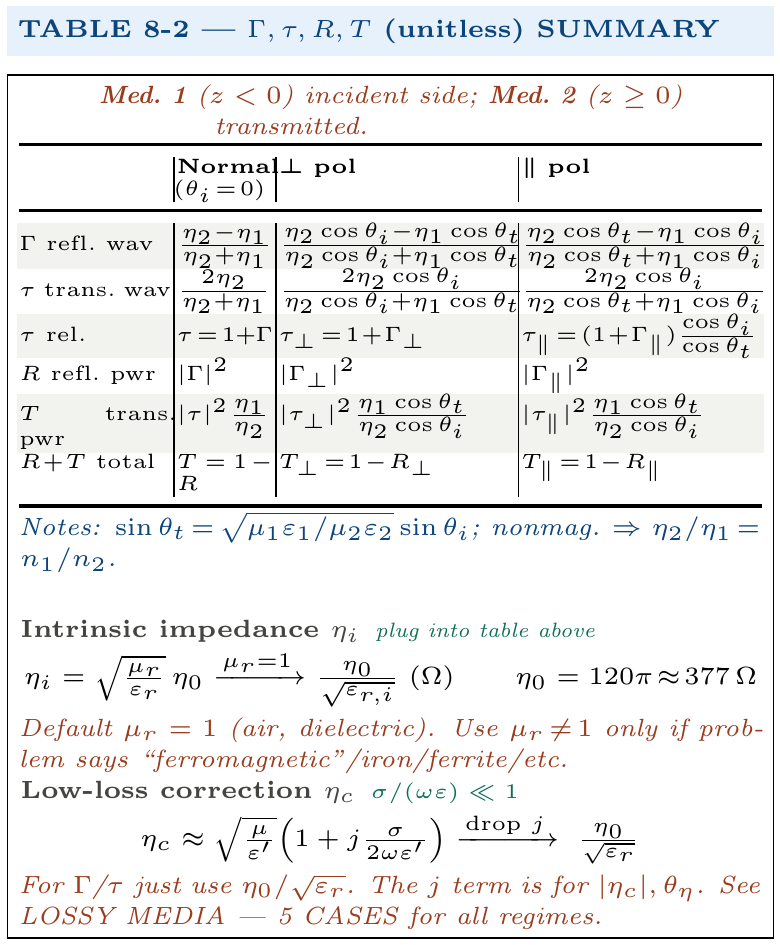
\includegraphics[width=0.49\linewidth]{cs_table82}\hfill
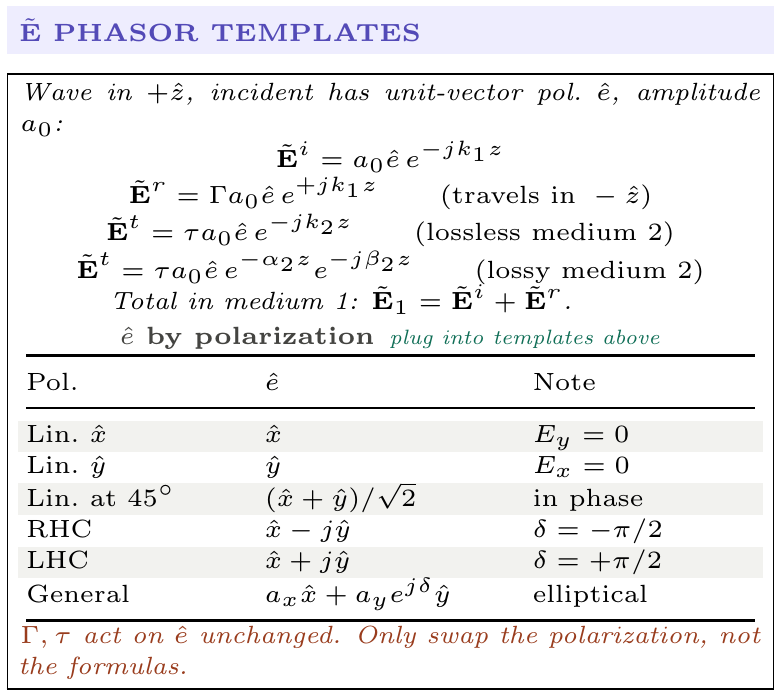
\includegraphics[width=0.49\linewidth]{cs_phasor_templates}\\[3pt]
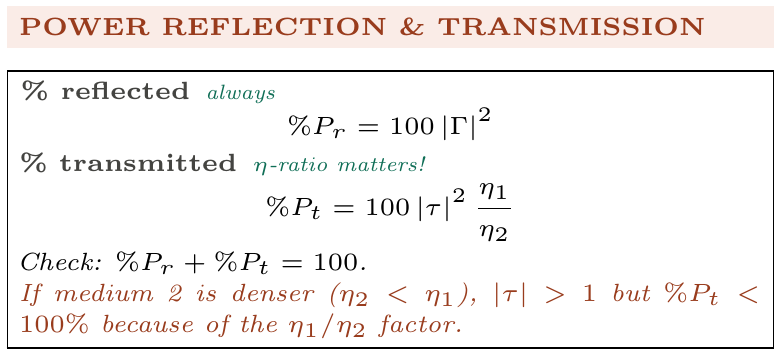
\includegraphics[width=0.49\linewidth]{cs_power}
\end{cssnip}

\textbf{(a) Incident E phasor.}\quad Template: $\tilde{\mathbf{E}}^i = a_0\hat{e}\,e^{-jk_1u}$.

\begin{minipage}[t]{0.55\linewidth}\vspace{0pt}
\[\tilde{\mathbf{E}}^i = 5(\hat{x}+j\hat{y})\,e^{-j(4\pi/3)z}\;\text{V/m}\]
\[\boxed{\tilde{\mathbf{E}}^i = 5(\hat{x}+j\hat{y})\,e^{-j4\pi z/3}\;\text{V/m}}\]
\end{minipage}\hfill
\begin{minipage}[t]{0.42\linewidth}\vspace{0pt}
\begin{givens}
\textbf{Givens:}\\
$f = 200$ MHz, $\omega = 2\pi f = 4\pi{\times}10^8$ rad/s\\
$u = z$;\ $\mu_r = \varepsilon_{r1} = 1$ (Air)\\
$\hat{e} = \hat{x}+j\hat{y}$ (LHC)\\
$k_1 = \omega\sqrt{\varepsilon_{r1}}/c = 4\pi/3$ rad/m\\
$c = 3{\times}10^8$ m/s;\ $a_0 = 5$ V/m
\end{givens}
\end{minipage}

\textbf{(b) Reflection \& transmission coefficients.}

\begin{minipage}[t]{0.55\linewidth}\vspace{0pt}
\[\eta_1(\text{Air}) = \sqrt{\tfrac{\mu_r}{\varepsilon_{r1}}}\,\eta_0 = \sqrt{1/1}(120\pi) = 120\pi\,\Omega\]
\[\eta_2(\text{med 2}) = \sqrt{\tfrac{\mu_r}{\varepsilon_{r2}}}\,\eta_0 = \sqrt{1/4}(120\pi) = 60\pi\,\Omega\]
\[\Gamma = \tfrac{\eta_2-\eta_1}{\eta_2+\eta_1} = \tfrac{60\pi-120\pi}{60\pi+120\pi} = \boxed{-\tfrac{1}{3}}\;(\text{unitless})\]
\[\tau = 1+\Gamma = 1-\tfrac{1}{3} = \boxed{\tfrac{2}{3}}\;(\text{unitless})\]
\end{minipage}\hfill
\begin{minipage}[t]{0.42\linewidth}\vspace{0pt}
\begin{givens}
\textbf{Givens:}\\
$\eta_0 = 120\pi\,\Omega \approx 377\,\Omega$
\end{givens}
\end{minipage}

\textbf{(c) Reflected, transmitted, total field.}

Templates: $\tilde{\mathbf{E}}^r = \Gamma a_0\hat{e}\,e^{+jk_1u}$,\quad $\tilde{\mathbf{E}}^t = \tau a_0\hat{e}\,e^{-jk_2u}$.

\begin{minipage}[t]{0.55\linewidth}\vspace{0pt}
\[\tilde{\mathbf{E}}^r = -\tfrac{1}{3}(5)(\hat{x}+j\hat{y})\,e^{+j(4\pi/3)z}\]
\[\boxed{\tilde{\mathbf{E}}^r = -\tfrac{5}{3}(\hat{x}+j\hat{y})\,e^{j4\pi z/3}\;\text{V/m}}\]
\[\tilde{\mathbf{E}}^t = \tfrac{2}{3}(5)(\hat{x}+j\hat{y})\,e^{-j(8\pi/3)z}\]
\[\boxed{\tilde{\mathbf{E}}^t = \tfrac{10}{3}(\hat{x}+j\hat{y})\,e^{-j8\pi z/3}\;\text{V/m}}\]
\[\tilde{\mathbf{E}}_T = \tilde{\mathbf{E}}^i + \tilde{\mathbf{E}}^r\]
\[\boxed{\tilde{\mathbf{E}}_T = 5(\hat{x}+j\hat{y})\!\left[e^{-j4\pi z/3} - \tfrac{1}{3}e^{j4\pi z/3}\right]\,\text{V/m}}\]
\end{minipage}\hfill
\begin{minipage}[t]{0.42\linewidth}\vspace{0pt}
\begin{givens}
\textbf{Givens:}\\
$k_2 = \omega\sqrt{\varepsilon_{r2}}/c = 8\pi/3$\\
$\varepsilon_{r2} = 4$;\ $c = 3{\times}10^8$\\
$\omega = 400\pi{\times}10^6$
\end{givens}
\end{minipage}

\textbf{(d) \% reflected and transmitted power.}
\[\%P_r = 100|\Gamma|^2 = 100|{-}\tfrac{1}{3}|^2 = \boxed{11.1\%}\]
\[\%P_t = 100|\tau|^2\,\tfrac{\eta_1}{\eta_2} = 100|\tfrac{2}{3}|^2\,\tfrac{120\pi}{60\pi} = \boxed{88.9\%}\]
\textit{Check: $11.1\% + 88.9\% = 100\%$. Energy conserved $\checkmark$}

\newpage
%======================================================
\probhead{2 --- Same Setup, Med 2 = Poor Conductor ($\varepsilon_r{=}2.25,\,\sigma{=}10^{-4}$)}{20 pts}

\textbf{Setup:} Replace medium 2 with poor conductor: $\varepsilon_r = 2.25$, $\mu_r = 1$, $\sigma = 10^{-4}$ S/m. Med 1 unchanged.

\begin{cssnip}
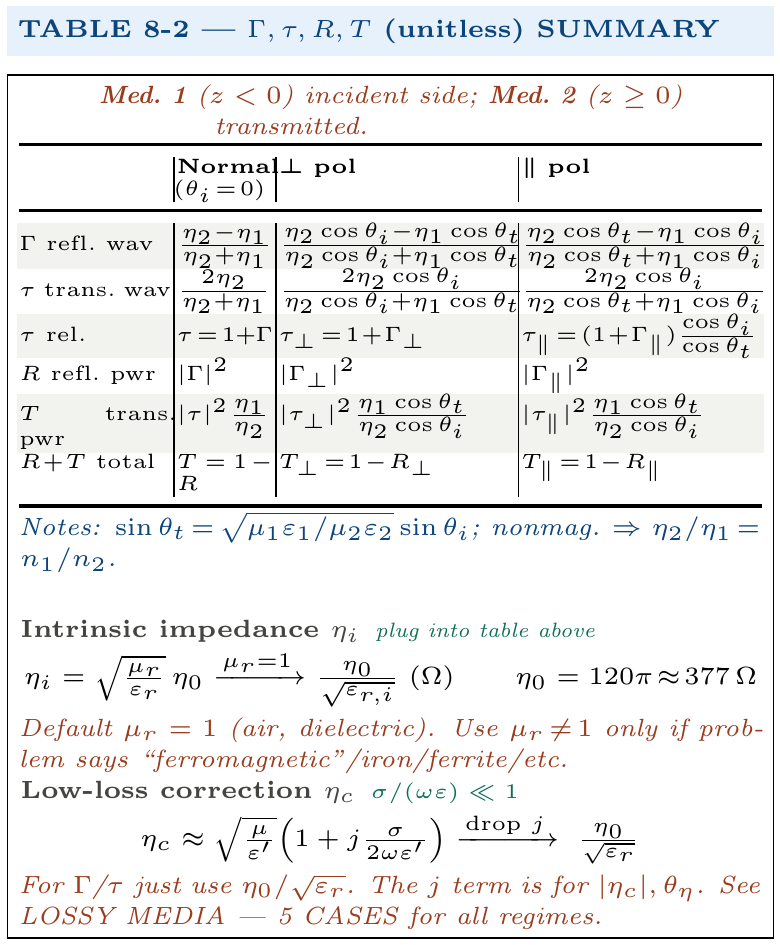
\includegraphics[width=0.49\linewidth]{cs_table82}\hfill
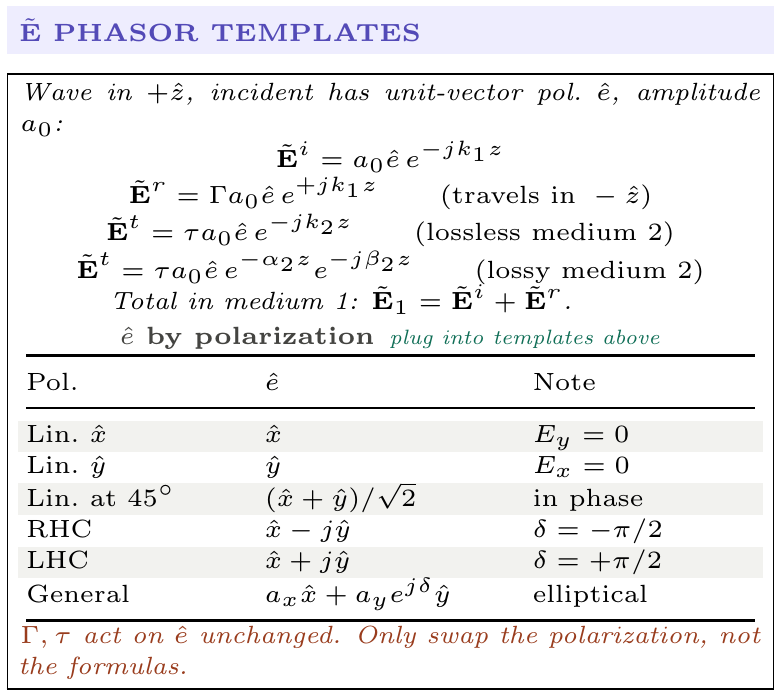
\includegraphics[width=0.49\linewidth]{cs_phasor_templates}\\[3pt]

\includegraphics[width=0.49\linewidth]{cs_lowloss}\hfill
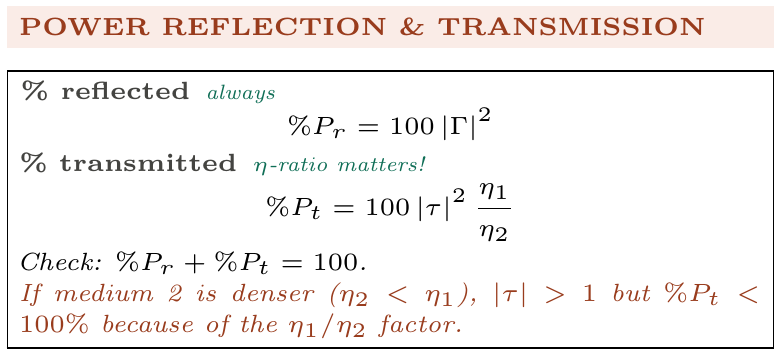
\includegraphics[width=0.49\linewidth]{cs_power}
\end{cssnip}

\textbf{(a) Incident E phasor.}\quad Med 1 didn't change, so same form as P1.
\[\boxed{\tilde{\mathbf{E}}^i = 5(\hat{x}+j\hat{y})\,e^{-j4\pi z/3}\;\text{V/m}}\]

\textbf{(b) Classify medium 2, then $\Gamma, \tau$.}

\begin{minipage}[t]{0.55\linewidth}\vspace{0pt}
Loss tangent:
\[\tfrac{\sigma}{\omega\varepsilon'} = \tfrac{10^{-4}}{(4\pi{\times}10^8)(2.25)(8.85{\times}10^{-12})} = 3.99{\times}10^{-3}\]
Since $\sigma/\omega\varepsilon' \ll 10^{-2}$, \textbf{low-loss}; use $\eta_0/\sqrt{\varepsilon_r}$.
\[\eta_1 = 120\pi\,\Omega,\quad \eta_2 = \tfrac{120\pi}{\sqrt{2.25}} = 80\pi\,\Omega\]
\[\Gamma = \tfrac{80\pi-120\pi}{80\pi+120\pi} = \boxed{-\tfrac{1}{5}}\;(\text{unitless})\]
\[\tau = 1+\Gamma = 1-\tfrac{1}{5} = \boxed{\tfrac{4}{5}}\;(\text{unitless})\]
\end{minipage}\hfill
\begin{minipage}[t]{0.42\linewidth}\vspace{0pt}
\begin{givens}
\textbf{Givens (med 2):}\\
$\varepsilon_{r2} = 2.25,\ \mu_{r2} = 1$\\
$\sigma_2 = 10^{-4}$ S/m\\
$\varepsilon_0 = 8.85{\times}10^{-12}$ F/m\\
$\omega = 400\pi{\times}10^6$ rad/s\\
$\eta_0 = 120\pi\,\Omega$
\end{givens}
\end{minipage}

\textbf{(c) Reflected, transmitted (lossy), total field.}

\begin{minipage}[t]{0.55\linewidth}\vspace{0pt}
\[\tilde{\mathbf{E}}^r = \Gamma a_0\hat{e}\,e^{+jk_1z} = -\tfrac{1}{5}(5)(\hat{x}+j\hat{y})e^{+j4\pi z/3}\]
\[\boxed{\tilde{\mathbf{E}}^r = -(\hat{x}+j\hat{y})\,e^{j4\pi z/3}\;\text{V/m}}\]
$\tilde{\mathbf{E}}^t$ replaces $e^{-jk_2z}$ with $e^{-\alpha_2 z}e^{-j\beta_2 z}$ (lossy):
\[\tilde{\mathbf{E}}^t = \tau a_0\hat{e}\,e^{-\alpha_2 z}e^{-j\beta_2 z} = \tfrac{4}{5}(5)(\hat{x}+j\hat{y})e^{-0.004\pi z}e^{-j2\pi z}\]
\[\boxed{\tilde{\mathbf{E}}^t = 4(\hat{x}+j\hat{y})\,e^{-0.004\pi z}e^{-j2\pi z}\;\text{V/m}}\]
\[\boxed{\tilde{\mathbf{E}}_T = 5(\hat{x}+j\hat{y})\!\left[e^{-j4\pi z/3} - \tfrac{1}{5}e^{j4\pi z/3}\right]\,\text{V/m}}\]
\end{minipage}\hfill
\begin{minipage}[t]{0.42\linewidth}\vspace{0pt}
\begin{givens}
\textbf{Low-loss row (Table 5-cases):}\\
$\alpha_2 \!\approx\! \tfrac{\sigma\eta_0}{2\sqrt{\varepsilon_r}} \!=\! \tfrac{10^{-4}(120\pi)}{2\sqrt{2.25}} \!=\! 0.004\pi$\\
\hspace*{0.7cm}$= 1.26{\times}10^{-2}$ Np/m\\
$\beta_2 \!\approx\! \tfrac{\omega\sqrt{\varepsilon_r}}{c} \!=\! \tfrac{(400\pi{\times}10^6)(1.5)}{3{\times}10^8} \!=\! 2\pi$ rad/m
\end{givens}
\end{minipage}

\textbf{(d) \% reflected and transmitted power.}
\[\%P_r = 100|\Gamma|^2 = 100|{-}\tfrac{1}{5}|^2 = \boxed{4\%}\]
\[\%P_t = 100|\tau|^2\,\tfrac{\eta_1}{\eta_2} = 100|\tfrac{4}{5}|^2\,\tfrac{120\pi}{80\pi} = \boxed{96\%}\]
\textit{Check: $4\% + 96\% = 100\%$. Energy conserved $\checkmark$}

\newpage
%======================================================
\probhead{3 --- Parallel-Pol, Two Layers ($\varepsilon_r{=}6.25, 2.25$)}{10 pts}

\textbf{Setup:} $\theta_i = 30^\circ$ from air into layer 1 ($\varepsilon_r = 6.25$, 5 cm), layer 2 ($\varepsilon_r = 2.25$, 5 cm), exits to air.

\begin{cssnip}
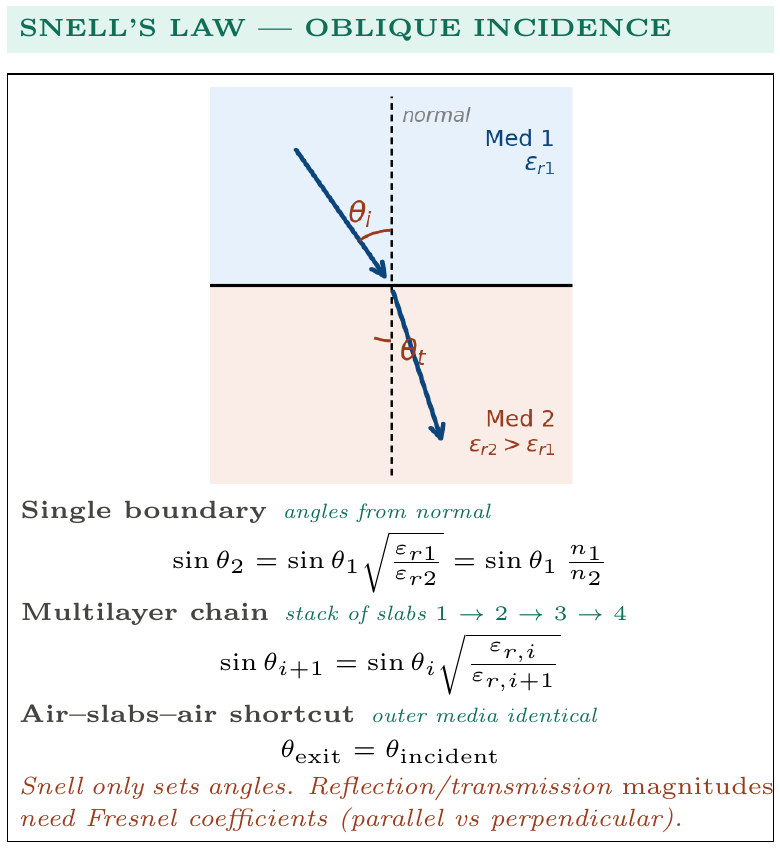
\includegraphics[width=0.49\linewidth]{cs_snell}\hfill
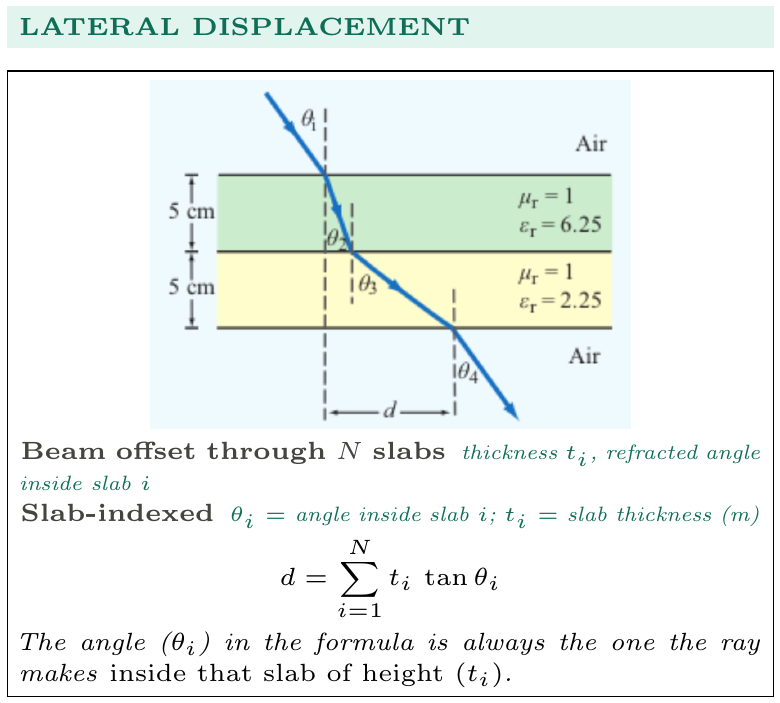
\includegraphics[width=0.49\linewidth]{cs_lateral}
\end{cssnip}

\textbf{(a) Chained Snell's law: $\sin\theta_{i+1} = \sin\theta_i\sqrt{\varepsilon_{r,i}/\varepsilon_{r,i+1}}$}

\begin{minipage}[t]{0.55\linewidth}\vspace{0pt}
\[\sin\theta_2 = \sin 30^\circ\sqrt{1/6.25} = 0.5(0.4) = 0.2\]
\[\boxed{\theta_2 = \sin^{-1}(0.2) = 11.54^\circ}\]
\[\sin\theta_3 = \sin\theta_2\sqrt{6.25/2.25} = 0.2(5/3) = 1/3\]
\[\boxed{\theta_3 = \sin^{-1}(1/3) = 19.47^\circ}\]
\[\sin\theta_4 = \sin\theta_3\sqrt{2.25/1} = (1/3)(1.5) = 0.5\]
\[\boxed{\theta_4 = 30.00^\circ = \theta_i}\]
\end{minipage}\hfill
\begin{minipage}[t]{0.42\linewidth}\vspace{0pt}
\begin{givens}
\textbf{Givens:}\\
$\varepsilon_{r1} = 1$ (air, $\theta_1 = 30^\circ$)\\
$\varepsilon_{r2} = 6.25$ (layer 1)\\
$\varepsilon_{r3} = 2.25$ (layer 2)\\
$\varepsilon_{r4} = 1$ (air exit)
\end{givens}
\end{minipage}

\textbf{(b) Lateral distance $d = \sum_i t_i\tan\theta_{\text{inside slab }i}$:}

\begin{minipage}[t]{0.55\linewidth}\vspace{0pt}
\[d = t_2\tan\theta_2 + t_3\tan\theta_3\]
\[= 0.05\tan(11.54^\circ) + 0.05\tan(19.47^\circ)\]
\[= 0.05(0.2041) + 0.05(0.3534)\]
\[\boxed{d = 0.0279\;\text{m} = 2.79\;\text{cm}}\]
\end{minipage}\hfill
\begin{minipage}[t]{0.42\linewidth}\vspace{0pt}
\begin{givens}
\textbf{Givens:}\\
$t_2 = t_3 = 0.05$ m (slab thickness)\\
$\theta_2 = 11.54^\circ$ (inside layer 1)\\
$\theta_3 = 19.47^\circ$ (inside layer 2)
\end{givens}
\end{minipage}

\newpage
%======================================================
\probhead{4 --- TE Waveguide, Find Mode, $\varepsilon_r$, $f_c$, $H_y$}{20 pts}

\textbf{Setup:} TE wave, $a = 5$ cm, $b = 3$ cm,
$E_x = -36\cos(40\pi x)\sin(100\pi y)\sin\!\big((2.4\pi{\times}10^{10})t - 52.9\pi z\big)$ V/m.

\begin{cssnip}
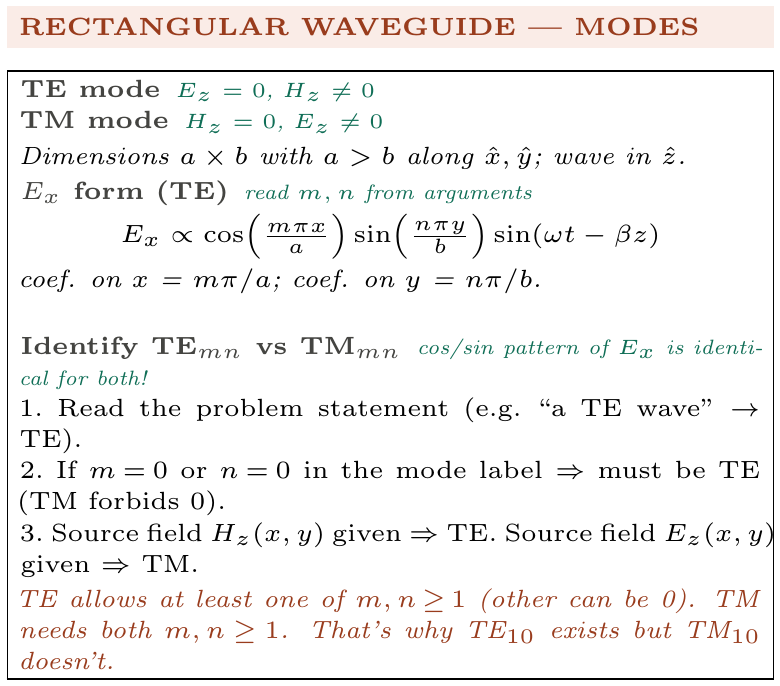
\includegraphics[width=0.49\linewidth]{cs_wgmodes}\hfill
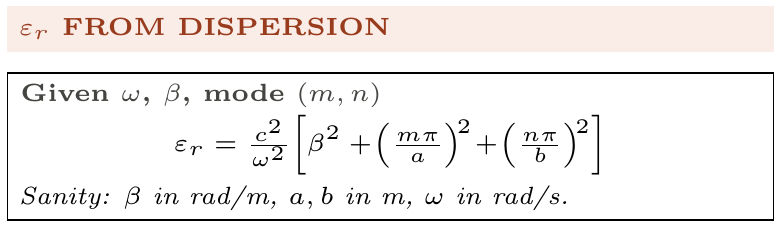
\includegraphics[width=0.49\linewidth]{cs_epsilon_disp}\\[3pt]
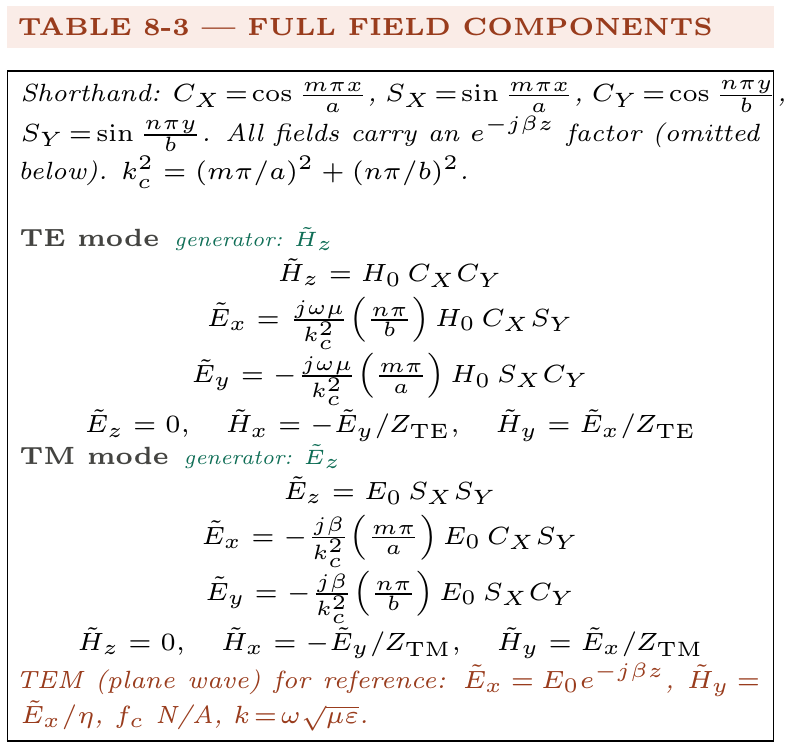
\includegraphics[width=0.95\linewidth]{cs_table83}
\end{cssnip}

\textit{\color{coral}New: Table 8-3 now contains $Z_\text{TE}/Z_\text{TM}$, full TEM column, and Properties Common ($f_c$, $\beta$, $u_p$, $u_{p0}$) --- one stop for all waveguide field formulas.}

\textbf{(a) Mode number.} Match $E_x$ to Table 8-3 TE-row form $\cos(m\pi x/a)\sin(n\pi y/b)$.

\begin{minipage}[t]{0.55\linewidth}\vspace{0pt}
\[\tfrac{m\pi}{a} = 40\pi \Rightarrow m = 40(0.05) = 2\]
\[\tfrac{n\pi}{b} = 100\pi \Rightarrow n = 100(0.03) = 3\]
\[\boxed{\text{Mode: TE}_{23}}\]
\end{minipage}\hfill
\begin{minipage}[t]{0.42\linewidth}\vspace{0pt}
\begin{givens}
\textbf{Givens:}\\
$a = 0.05$ m,\ $b = 0.03$ m\\
TE wave (given), so $E_z = 0$
\end{givens}
\end{minipage}

\textbf{(b) $\varepsilon_r$ from $\varepsilon_r$ FROM DISPERSION box (Example 8-8).}

\begin{minipage}[t]{0.55\linewidth}\vspace{0pt}
\[\varepsilon_r = \tfrac{c^2}{\omega^2}\!\left[\beta^2 + \!\left(\tfrac{m\pi}{a}\right)^{\!2}\!+\!\left(\tfrac{n\pi}{b}\right)^{\!2}\right]\]
\[= \!\left(\tfrac{3{\times}10^8}{2.4\pi{\times}10^{10}}\right)^{\!2}\!\big[(52.9\pi)^2 + (40\pi)^2 + (100\pi)^2\big]\]
\[\boxed{\varepsilon_r = 2.25}\]
\end{minipage}\hfill
\begin{minipage}[t]{0.42\linewidth}\vspace{0pt}
\begin{givens}
\textbf{Givens:}\\
$\beta = 52.9\pi$ rad/m\\
$\omega = 2.4\pi{\times}10^{10}$ rad/s\\
$c = 3{\times}10^8$ m/s
\end{givens}
\end{minipage}

\textbf{(c) Cutoff frequency for TE$_{23}$ from Table 8-3 Properties Common.}

\begin{minipage}[t]{0.55\linewidth}\vspace{0pt}
\[u_{p0} = \tfrac{c}{\sqrt{\varepsilon_r}} = \tfrac{3{\times}10^8}{1.5} = 2{\times}10^8\;\text{m/s}\]
\[f_{23} = \tfrac{u_{p0}}{2}\sqrt{\!\left(\tfrac{m}{a}\right)^{\!2}\!+\!\left(\tfrac{n}{b}\right)^{\!2}}\]
\[= 10^8\sqrt{(2/0.05)^2 + (3/0.03)^2} = 10^8\sqrt{11600}\]
\[\boxed{f_c = 10.77\;\text{GHz}}\]
\end{minipage}\hfill
\begin{minipage}[t]{0.42\linewidth}\vspace{0pt}
\begin{givens}
\textbf{Givens:}\\
$m = 2,\ n = 3$\\
$a = 0.05,\ b = 0.03$ m\\
$\varepsilon_r = 2.25$ (from b)
\end{givens}
\end{minipage}

\textbf{(d) $H_y$ from Table 8-3 TE block: $\tilde{H}_y = \tilde{E}_x/Z_\text{TE}$.}

\begin{minipage}[t]{0.55\linewidth}\vspace{0pt}
\[\eta = \tfrac{\eta_0}{\sqrt{\varepsilon_r}} = \tfrac{120\pi}{\sqrt{2.25}} = 80\pi\,\Omega\]
\[Z_\text{TE} = \tfrac{\eta}{\sqrt{1-(f_c/f)^2}} = \tfrac{80\pi}{\sqrt{1-(10.77/12)^2}} = 569.9\,\Omega\]
\[H_y = \tfrac{E_x}{Z_\text{TE}} = \tfrac{-36}{569.9}\cos(40\pi x)\sin(100\pi y)\sin(\omega t-\beta z)\]
\[\boxed{H_y = -0.0632\cos(40\pi x)\sin(100\pi y)\sin\!\big((2.4\pi{\times}10^{10})t-52.9\pi z\big)\;\text{A/m}}\]
\end{minipage}\hfill
\begin{minipage}[t]{0.42\linewidth}\vspace{0pt}
\begin{givens}
\textbf{Givens:}\\
$f = \omega/(2\pi) = 12$ GHz\\
$f_c = 10.77$ GHz\\
$\eta_0 = 120\pi \approx 377\,\Omega$\\
$\varepsilon_r = 2.25$
\end{givens}
\end{minipage}

\newpage
%======================================================
\probhead{5 --- Hollow Guide Multi-Mode Travel Times}{8 pts}

\textbf{Setup:} Hollow guide ($\varepsilon_r = 1$, $u_{p0} = c$), $a = 3$ cm, $b = 2$ cm. Carrier 9.5 GHz, length $L = 100$ m. Find $t$ for each excited mode.

\begin{cssnip}
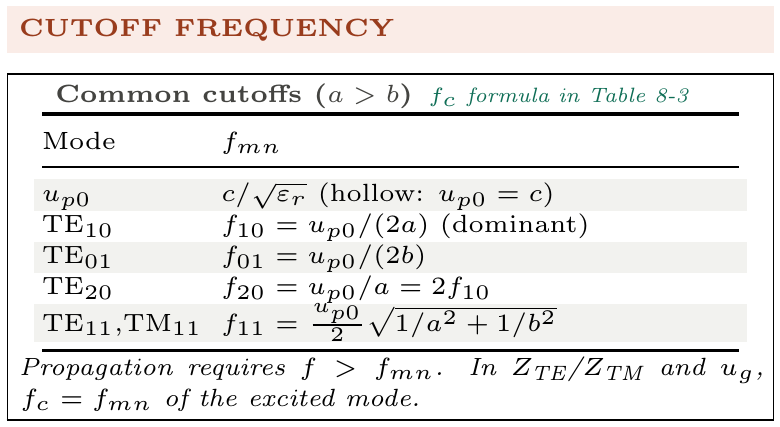
\includegraphics[width=0.49\linewidth]{cs_cutoff}\hfill
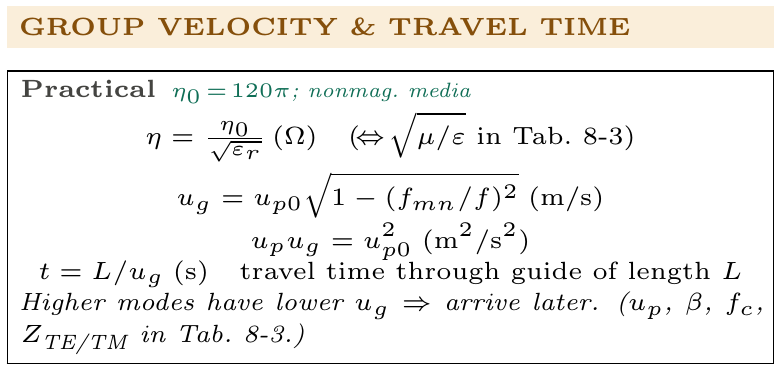
\includegraphics[width=0.49\linewidth]{cs_groupvel}
\end{cssnip}

\textbf{Cutoffs (compute lowest modes, stop when $f_{mn} > 9.5$ GHz):}

\begin{minipage}[t]{0.55\linewidth}\vspace{0pt}
\[f_{10} = \tfrac{c}{2a} = \tfrac{3{\times}10^8}{0.06} = 5\;\text{GHz}\quad(<\!9.5,\text{ excited})\]
\[f_{01} = \tfrac{c}{2b} = \tfrac{3{\times}10^8}{0.04} = 7.5\;\text{GHz}\quad(<\!9.5,\text{ excited})\]
\[f_{20} = \tfrac{c}{a} = 10\;\text{GHz}\quad(>\!9.5,\text{ not excited})\]
\[f_{11} = \tfrac{c}{2}\sqrt{\tfrac{1}{a^2}+\tfrac{1}{b^2}} = 9.014\;\text{GHz}\quad(<\!9.5,\text{ excited})\]
\end{minipage}\hfill
\begin{minipage}[t]{0.42\linewidth}\vspace{0pt}
\begin{givens}
\textbf{Givens:}\\
$f = 9.5$ GHz (carrier)\\
$a = 0.03,\ b = 0.02$ m\\
$u_{p0} = c$ (hollow)\\
$L = 100$ m
\end{givens}
\end{minipage}

\textbf{Travel times: $u_g = u_{p0}\sqrt{1-(f_{mn}/f)^2}$, $t = L/u_g$.}

\begin{center}
\begin{tabular}{lccc}
\toprule
Mode & $f_c$ (GHz) & $u_g$ (m/s) & $t = L/u_g$\\
\midrule
\rowcolor{purplebg!50} TE$_{10}$ & 5.000 & $3{\times}10^8\sqrt{1-(5/9.5)^2} = 2.551{\times}10^8$ & $\boxed{0.392\;\mu\text{s}}$\\
TE$_{01}$ & 7.500 & $3{\times}10^8\sqrt{1-(7.5/9.5)^2} = 1.841{\times}10^8$ & $\boxed{543.1\;\text{ns}}$\\
\rowcolor{purplebg!50} TE$_{20}$ & 10.000 & N/A (not excited) & N/A\\
TE$_{11}$, TM$_{11}$ & 9.014 & $3{\times}10^8\sqrt{1-(9.014/9.5)^2} = 9.510{\times}10^7$ & $\boxed{1.05\;\mu\text{s}}$\\
\bottomrule
\end{tabular}
\end{center}

\textit{Higher modes arrive later: as $f_{mn} \to f$, $u_g \to 0$, so closer-to-cutoff modes have longer travel time.}

\end{document}
